\documentclass[a4paper,12pt]{scrreprt}
\usepackage[ngerman]{babel}
\usepackage[left=2cm,right=2cm,top=2.5cm,bottom=2.5cm]{geometry}
\usepackage{amsmath}
\usepackage{acronym}
\usepackage{amsfonts}
\usepackage{amssymb}
\usepackage{makeidx}
\usepackage{graphicx}
\usepackage{epstopdf}
\usepackage{kpfonts}
\usepackage[onehalfspacing]{setspace}
\usepackage[colorlinks=true, allcolors=blue]{hyperref}
\usepackage[backend=biber,style=apa]{biblatex}
\addbibresource{references.bib}
\newcommand{\dcplace}{Aachen}
\newcommand{\dcdate}{04. Mai 2025}
\newcommand{\dcauthorfirstname}{Max}
\newcommand{\dcauthorlastname}{Mustermann}

\usepackage{fancyhdr}
\pagestyle{fancy}
\fancyhf{}
\fancyhead[L]{\nouppercase{\leftmark}} % Kapitelname in normaler Schrift
\fancyhead[R]{} 
\setlength{\parindent}{0pt}
\fancyfoot[C]{\thepage} 

\usepackage{listings}
\usepackage{xcolor}
\definecolor{bggray}{gray}{0.95}
\definecolor{codeblue}{rgb}{0.1, 0.1, 0.8}
\definecolor{codered}{rgb}{0.8, 0.1, 0.1}
\definecolor{codegreen}{rgb}{0.1, 0.6, 0.1}
\definecolor{codeorange}{rgb}{0.9, 0.5, 0.1}
\lstset{
    basicstyle=\ttfamily\small\color{codeblue},
    backgroundcolor=\color{bggray},
    keywordstyle=\color{codered}\bfseries,
    stringstyle=\color{codegreen}, 
    commentstyle=\color{gray}\itshape, 
    breaklines=true, 
    showspaces=false,
    showstringspaces=false,
    showtabs=false,
    tabsize=2
}
\lstdefinelanguage{properties}{
    morecomment=[l]{\#},
    morecomment=[s]{/*}{*/},
    morestring=[b]",
    basicstyle=\ttfamily\small\color{codeblue},
    keywordstyle=\color{codeorange}\bfseries,
    commentstyle=\color{codegreen}\itshape,
    backgroundcolor=\color{bggray},
    breaklines=true,
    showspaces=false,
    showstringspaces=false,
    showtabs=false,
    tabsize=2
}
\lstdefinelanguage{POM}{
    language=XML,
    basicstyle=\ttfamily\small\color{codeblue},
    keywordstyle=\color{codeorange}\bfseries,
    stringstyle=\color{codegreen},
    backgroundcolor=\color{bggray},
    morekeywords={dependency, groupId, artifactId, version, dependencies},
    breaklines=true,
    showspaces=false,
    showstringspaces=false,
    showtabs=false,
    tabsize=2
}


\begin{document}
\begin{titlepage}
	%ab hier kleinere Raender, mehr bedruckbare Flaeche.
	\thispagestyle{empty}
	\newgeometry{a4paper, portrait, left=1.0cm, right=0cm, top=0.6cm, bottom=0cm, includefoot}

    \noindent
    \begin{minipage}[t]{0.5\textwidth}
        
\includegraphics[width=3.7cm]{firmenlogo.jpg}
    \end{minipage}%
    \begin{minipage}[t]{0.5\textwidth}
          \raggedleft
          
\includegraphics[width=1.7cm]{FHAC.jpg}
    \end{minipage}

	\vspace{1.0cm}

	% Kopfzeile mit Fachbereich ...
	{\centering \bfseries \Large FH~Aachen \\
	\vspace{1cm}
	\normalsize Fachbereich\\
	Elektrotechnik und Informationstechnik \\
	Studiengang~Informatik \par}

	\vspace{1cm}
    
	{\centering \bfseries \large Bachelorarbeit \par}

	\vspace{1cm}

	\centering \begin{minipage}[t]{13cm}
		\centering \small Konzeption und prototypische Entwicklung einer webbasierten Applikation zur Wertschöpfung und Bereitstellung von Geodaten \\
        (Data-Konnector für Geodaten)
		\medskip
	\end{minipage}

	\vspace{1.5cm}
    
	%\vspace*{1cm}
	%\hspace*{6.8cm}
	\begin{minipage}[t]{9cm}
		\centering Tuan Anh Cong Nguyen \\ Matr.-Nr.: 3517392
	\end{minipage}
	\vspace{2.1cm}
    
	%\vspace*{4.7cm}
	%\hspace*{6.8cm}
	\centering \begin{minipage}[b]{15cm}
		\centering
			Referent: Prof. Dr. rer. nat. Heinrich Faßbender\\
			%Korreferent: Prof. Dr.-Ing. ...\
	\end{minipage}


	\vspace{1.5cm}
	
	%Erstellungsdatum
	%\vspace{-4cm}
	%\begin{flushright}
	\centering %\hspace{8cm}
	\begin{minipage}[b]{10cm}
			\centering
            In Zusammenarbeit mit Ausbildungsbetrieb:\\
            ahu GmbH Wasser Boden Geomatik \\
            \vspace{1cm}
            Externer Betreuer: Dr. David Loibl
            
			%\today\\ %Datum\\
			%\vspace{1cm}
			%vertraulich bis xx.xx.xx
	\end{minipage}
	%\end{flushright}

	%\today
	\restoregeometry
\end{titlepage}

\clearpage % Neue Seite für Selbstständigkeitserklärung
\chapter*{Selbstständigkeitserklärung}
\thispagestyle{empty}	%keine Seitenzahl!
\pdfbookmark{Selbstständigkeitserklärung}{Selbstständigkeitserklärung}
Ich versichere hiermit, dass ich die vorliegende Arbeit selbständig verfasst und keine anderen als die im Literaturverzeichnis angegebenen Quellen benutzt habe.\\ \\
Stellen, die wörtlich oder sinngemäß aus veröffentlichten oder noch nicht veröffentlichten Quellen entnommen sind, sind als solche kenntlich gemacht.\\ \\ Die Zeichnungen oder Abbildungen in dieser Arbeit sind von mir selbst erstellt worden oder mit einem entsprechenden Quellennachweis versehen.\\ \\ Diese Arbeit ist in gleicher oder ähnlicher Form noch bei keiner anderen Prüfungsbehörde eingereicht worden.\\ \\[2ex]
Aachen, den \today \hspace{4cm} \dotfill 
\tableofcontents

\clearpage
\chapter*{Abkürzungsverzeichnis}\label{abkuerzungsverzeichnis}
\begin{acronym}[YTM]
\setlength{\itemsep}{-\parsep}

\acro{REST-API}{\hspace{1cm}Representational State Transfer Application Program Interface}
\acro{Nu}[$Nu$]{\hspace{1cm}Nußelt-Zahl}
\acro{nu_luft}[$\nu_{Luft}$]{\hspace{1cm}Kinematische Viskosität von Luft}
\acro{Pr}[$Pr$]{\hspace{1cm}Prandtl-Zahl}
\acro{Q}[$\dot Q$]{\hspace{1cm}Wärmestrom}
\acro{Ra}[$Ra$]{\hspace{1cm}Rayleigh-Zahl}
\acro{rho_luft}[$\rho_{Luft}$]{\hspace{1cm}Dichte von Luft}
\acro{temperatur}[$T$]{\hspace{1cm}Temperatur}
\acro{umgebungstemperatur}[$T_{\infty}$]{\hspace{1cm}Umgebungstemperatur}

\end{acronym}

\cleardoublepage
\chapter*{Abstract}
\thispagestyle{plain}
\addcontentsline{toc}{chapter}{Abstract}
In einer zunehmend digitalisierten und automatisierten Welt wächst täglich die Menge an neu generierten Geodaten – insbesondere Mess- und räumlichen Daten.\\ \\
Die Suche nach und Einbindung von OGC-Geodatendiensten wie WMS (Web Map Service) und WFS (Web Feature Service) in Geoinformationssysteme wie QGIS kann tatsächlich schwierig sein. Die Suche erfordert den Anwender oft das Durchforsten verschiedener Quellen und die manuelle Überprüfung von Dienstbeschreibung. Eine automatisiert und effiziente Lösung kann teilweise helfen, diesen Prozess zu verbessern. \\ 
Die Suche nach Messdaten wie Grundwasserständen, Pegelständen und Klimadaten (Niederschlag,Temperatur) und deren Umformatierung in ein einheitliches Format gestalten sich als schwierig und kompliziert, da es eine Vielzahl von Datenanbietern mit unterschiedliche Datenstrukturen, Formen, etc. gibt.\\ \\
Die Bereitstellung dieser Rohdaten erfolgt meinst im CSV-Format oder als individuell strukturierte ASCII-Dateien. Im Kontext von der Datenkonsum, gibt es bei der Ahu den sogenannten ahuManager-Client, der diese Daten konsumiert. Bevor diese konsumieren können, müssen die Rohdaten in ein kompatibles Format umformatiert werden, was bisher teilweise von Hand erledigt werden (in Excel o.ä.). Diese manuelle Vorgehen kann perspektivisch zum Teil oder ganz automatisiert werden, was die Produktivität steigert und die Fehleranfälligkeit vermeidet. \\ \\
Daher befasst sich diese Arbeit  mit dem Thema, wie eine webbasierte Applikation zur Wertschöpfung und Bereitstellung von rohen Geodaten im Kontext von der Abteilung Geomatik von Ahu GmbH entwickelt werden kann.

\clearpage
\chapter{Einleitung}
\section{Motivation der Arbeit}
Diese Bachelorarbeit wird in Zusammenarbeit mit dem Bereich Geomatik der Ahu GmbH verfasst.Der Bereich beschäftigt sich mit Konzeption und Softwareentwicklung der Monitoringsysteme und Web-Anwendungen, die es Dienstleitern, Betreibern und Aufsichtsbehörden ermöglichen, ein kosteneffizientes Management für Geodaten(Grundwasser, Oberflächenwasser, Boden,etc.) umzusetzen. \\ \\
Momentan besteht es Bedarf für ein zentrales System zur automatisierten Suche und Verwaltung der Geodaten aus verschiedenen Datenanbietern und diese Daten in einer homogen Struktur zusammenzubringen und einen vorhandenen Client(z.B ahuManager) bereitzustellen. Unter anderem  wird auch die Einbindung von OGC-Geodatendiensten für besseren und effizienten Prozess zur Durchsuche und Verwaltung gesorgt. 

\section{Ziel der Arbeit}
Die Hauptaufgabe dieser Arbeit besteht darin, ein Konzeption für die prototypische Entwicklung einer webbasierten Applikation zu erstellen und umzusetzen. Die Ziele enthalten eine übergreifende Suche von Geodaten und deren Umformatierung in ein passendes vorgegebenes Zielformat. Das weitere Zeil ist die Einbindung von mindestens einer OGC-Geodatendiensten.\\ \\ Durch die Umsetzungen dieser Ziele soll perspektivisch eine Software entstehen, die offene Problematik eine mögliche Lösung anbietet.

\section{Aufbau der Arbeit}
\section*{\small \textbf{Kapitel 1: Einleitung}}
Im ersten Kapitel werden die Motivation und Zwecke für diese Arbeit erklärt. Es wird kurz auf die Problematik des gewählten Themas eingegangen und dieses perspektivisch für die Firma auch Vorteile bringt.

\section*{\small \textbf{Kapitel 2: Übersicht von Technologien}}
In diesem Kapitel werden wichtige Begriffe und in der Entwicklungsphase verwendete Technologien vorgestellt. Von der Bibliothek zur Verfolgung der Datenbankänderungen über das Backend-Framework bis hin zu in der Benutzeroberfläche verwendetem UI-Framework.   
\section*{\small \textbf{Kapitel 3: Anforderungsanalyse und Spezifikation}}
Diese Kapitel 
\section*{\small \textbf{Kapitel 4: Konzeption und Architektur}}
Dieses Kapitel erläutert die angewandte Architektur des Prototyps anhand von unterschiedlichen Sichten.
\section*{\small \textbf{Kapitel 5: Implementierung}}
Anhand zahlreichen Code-Beispiele und technischen Erläuterungen wird die wirkliche Implementierung nochmal veranschaulicht. 
\section*{\small \textbf{Kapitel 6: Evaluierung}}
Das vorletzte Kapitel bewertet, inwiefern die vom Anfang festgelegte und erarbeitete Anforderungen erfüllt wurde. 
\section*{\small \textbf{Kapitel 7: Fazit und Ausblick für weitere Entwicklung}}
Abschließend wird noch einmal die gesamte Arbeit zusammenfassend bewertet und ein kurzer Ausblick für weiteren Entwicklungen oder Verbesserungen in der Zukunft gegeben.

\chapter{Übersicht von Technologien}
\section{Vaadin}
Vaadin ist ein serverseitiges Web-Framework, das dem Entwickler erlaubt, moderne Webanwendung in Java zu entwickeln, ohne dass explizit HTML,CSS oder JavaScript geschrieben werden muss. Vaddin verfügt über eine große Komponentenbibliothek, die eine Vielzahl an vorgefertigten UI-Elementen wie Buttons, Tabellen, Formulare, Dialoge und Layouts bietet.

\begin{figure}[h!]
\centering
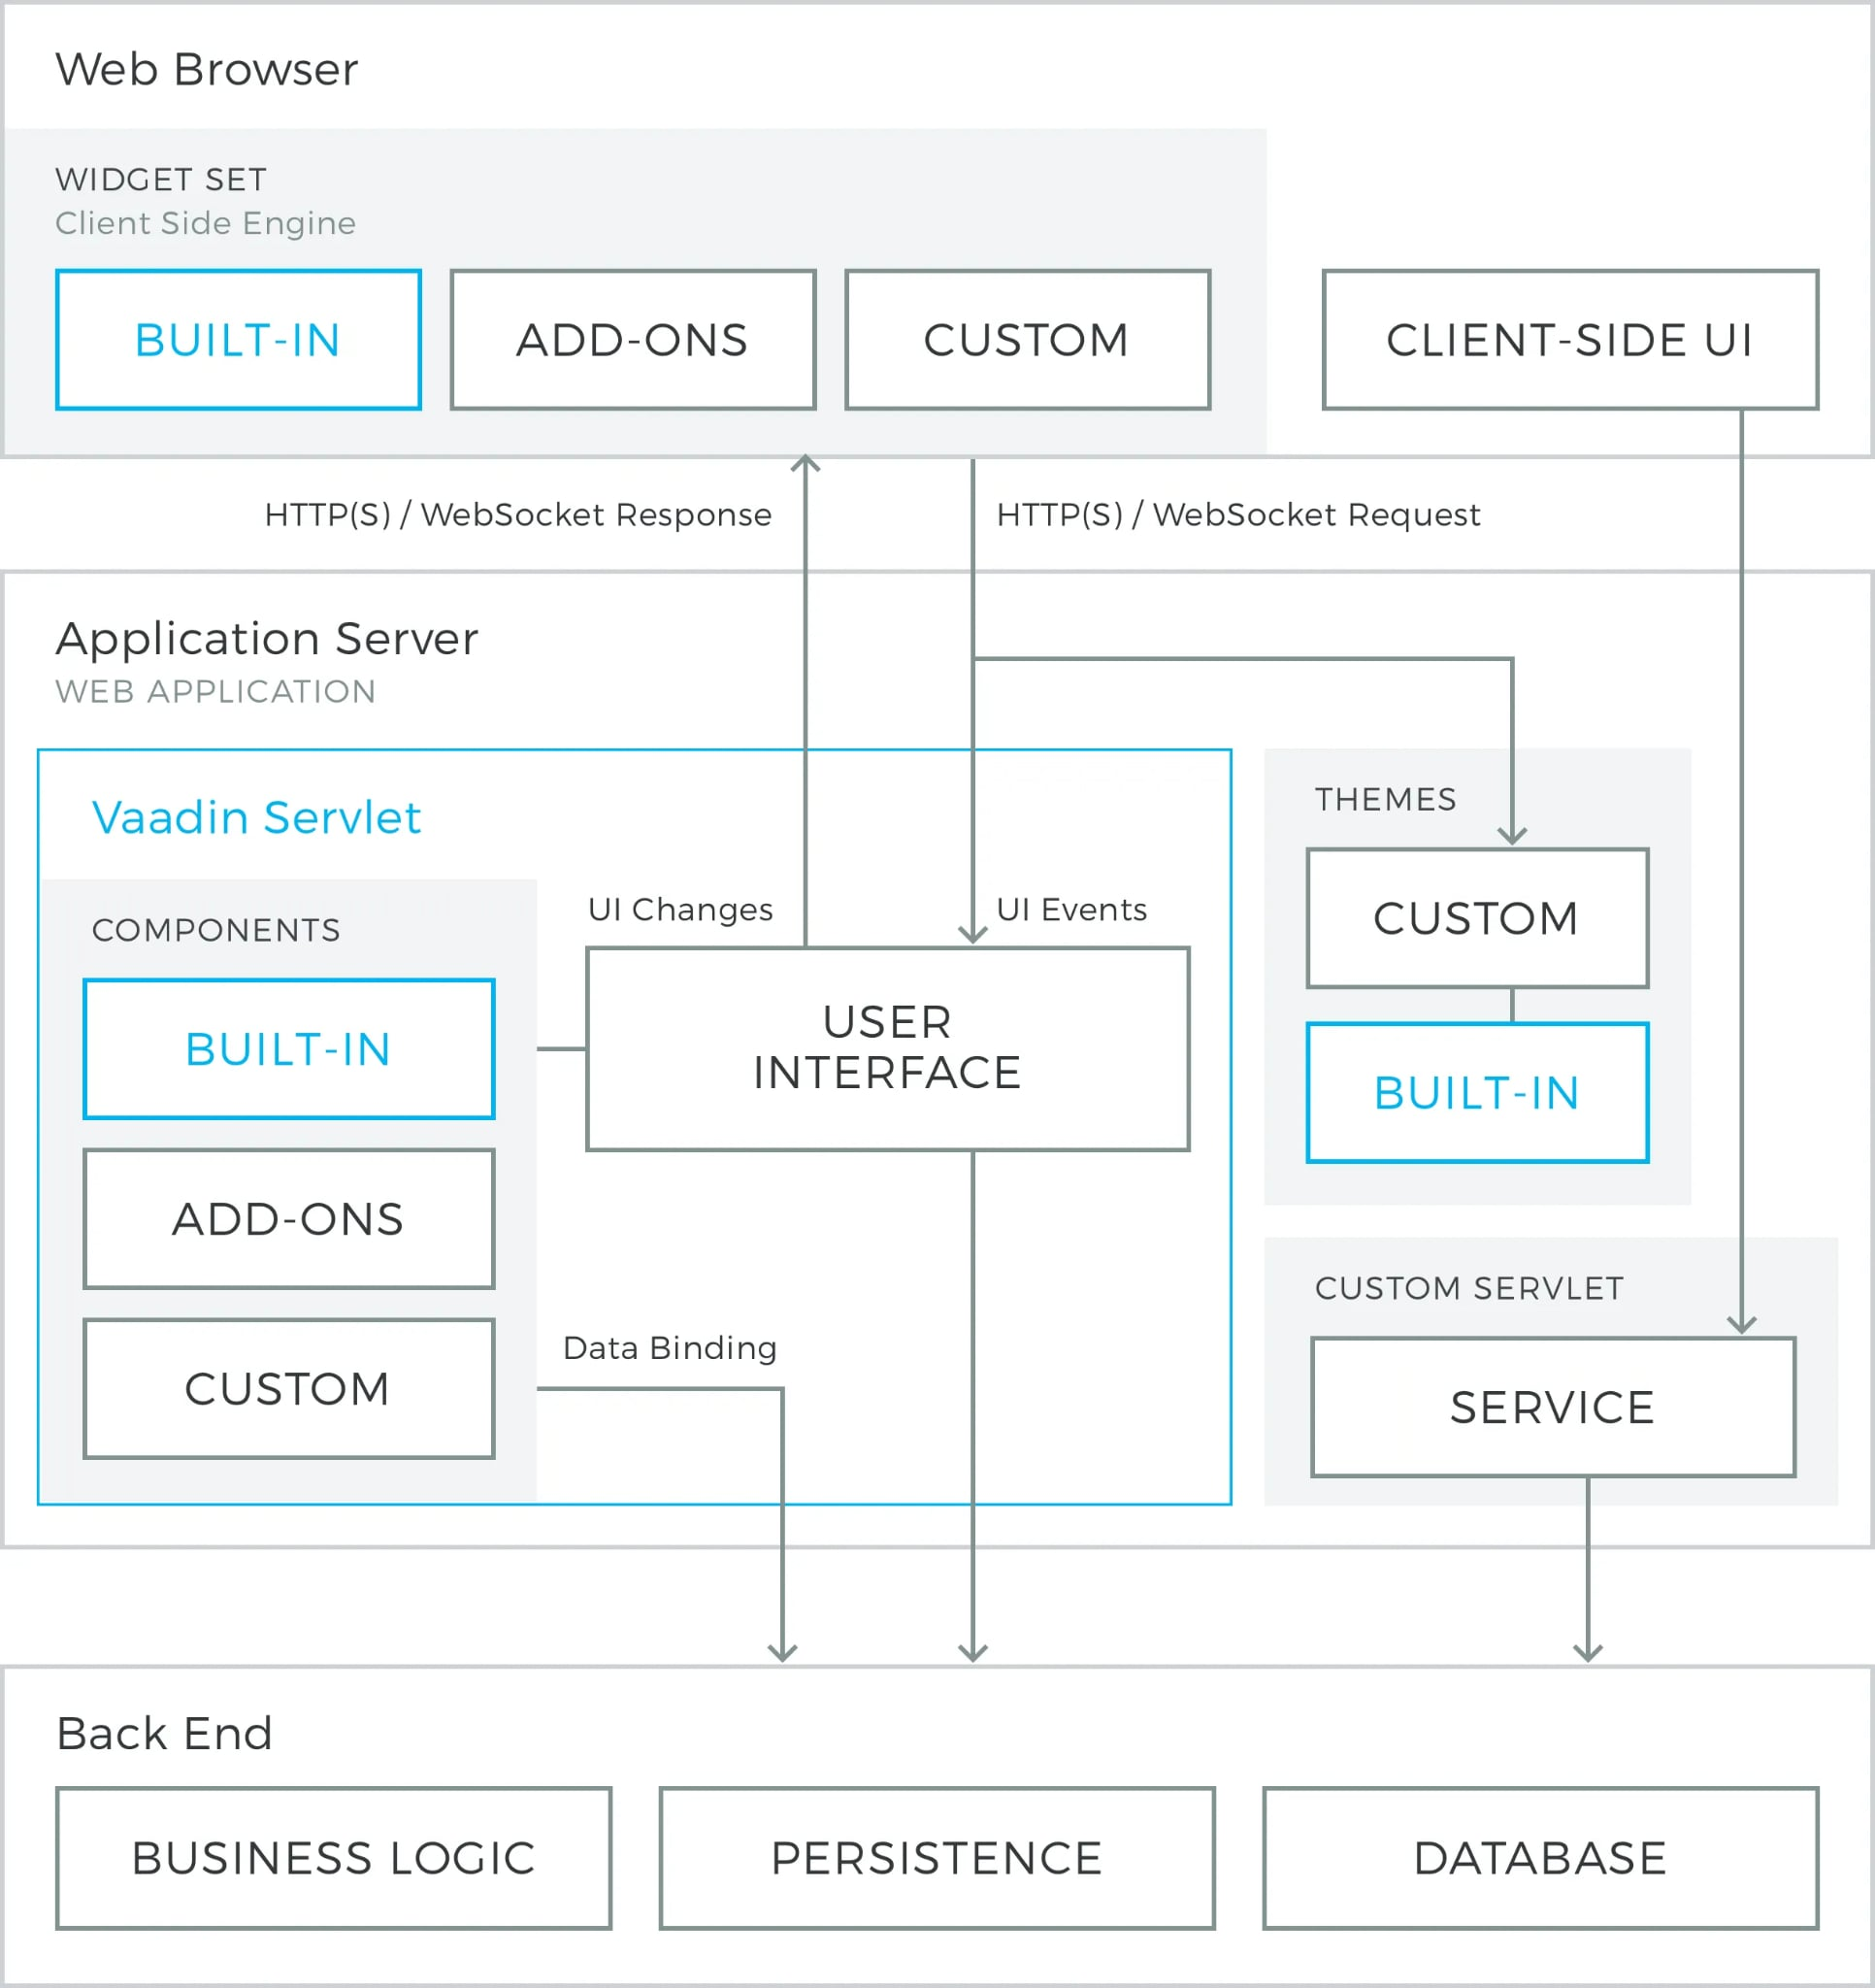
\includegraphics[width=9cm, height=10cm]{vaadin_architekture.jpg}
\caption{\label{vaadin:architektur}Übersicht Vaadin Architektur \cite{architecture21}}
\end{figure}
Vaadin verfolgt einen serverseitigen Rendering-Ansatz. Während eine AJAX-basierte Vaadin Client-Side Engine dafür sorgt, dass die Benutzeroberfläche im Browser durch ein Widget-Set gerendert wird. Die Benutzeroberfläche kann aus eingebauten Komponenten, Add-Ons und benutzerdefinierten Komponenten bestehen. Diese Client-Side Engine kommuniziert über HTTP oder WebSockets mit dem Server. Die gesamte UI-Logik wird dann auf dem Server ausgeführt. Die Vaadin Servlet empfängt Client-Anfragen und aktualisiert die Benutzeroberfläche. Die UI-Komponenten werden serverseitig erstellt und verwaltet. Änderungen in der UI werden durch die Vaddin Client-Side Engine an den Browser zurückgespielt.  

\section{Spring Framework}
Spring Framework ist ein Java-Framework, das um 2003 als Reaktion auf die damals noch zu komplizierte J2EE-Plattform entwickelt wurde. Spring ermöglicht eine einfachere und unkompliziertere Entwicklung von Enterprise-Applikation in Java. Eines der wichtigsten Konzepte von Spring war die Inversion of Control (IoC).
IoC ist ein Prinzip, bei dem der Kontrollfluss an eine externe Quelle(z.B. ein Framework) übergeben wird. Das Framework ist dann gemäß einer Spezifikation für die Erstellung und Löschung der Objekte und den Aufruf von Methoden verantwortlich. \\ \\ Spring führt das Konzept des Bean-Containers ein. Beans sind Java-Objekte, die von Spring instanziiert und verwaltet sind. Wenn die Haupt-Bean von der Hilfs-Bean abhängig ist, stellt Spring sicher, dass die Hilfs-Bean vor der Haupt-Bean initialisiert wird. Spring injizierte außerdem die Instanz der Hilfs-Bean in die Haupt-Bean, sodass die Haupt-Bean nicht mehr nach ihren eigenen Abhängigkeiten suchen muss. Dieses Muster wird als Dependendy Injection bezeichnet.\\ \\
Damals musste der Entwickler die Bean-Konfiguration in XML schreiben, die Spring anweist, wie die Beans zu konstruieren sind. Inzwischen wird diese mithilfe einer Kombination aus Java-Annotation, Java-Code und Konventionen erstellt.
\section{Spring Boot}
Mit dem Wachstum der Spring-Plattform nahm auch die Komplexität der Entwicklung von Spring-Anwendungen zu. Gleichzeitig verbreitet sich der Einsatz von Microservices und containerisierten Umgebungen in der Softwareentwicklung. Entwickler wünschten sich einfach Methode, um schlanke Webanwendungen zu erstellen, die unabhängig als eigenständige Dienst ausgeführt werden können, anstatt auf einem dedizierten Anwendungsserver zu laufen.\\ \\
Spring Boot wurde als Reaktion auf diese Anforderungen entwickelt. Es erleichtert die Erstellung von Spring-Anwendungen durch sinnvolle Standard-Einstellungen, Starter-Abhängigkeiten und produktionsreife Funktionen für Konfiguration und Überwachung. Durch die Einführung eingebetteter Servlet-Container wurde es möglich, Anwendungen als eigenständige, ausführbare JAR-Dateien zu verpacken. 
\section{Maven}
Maven ist ein Build-Management- und Projektverwaltungswerkzeug, das häufig in der Java-Entwicklung eingesetzt wird. Es automatisiert Aufgaben wie das Herunterladen von Abhängigkeiten, das Kompilieren von Quellcode und das Ausführen von Builds sowie Tests. Maven verwendet eine zentrale Konfigurationsdatei, die \texttt{pom.xml}, um alle Aspekte des Projekts wie Libraries, Plugins und Build-Prozesse zu steuern.\\ \\
Die Funktionsweise von Maven basiert auf einem deklarativen Ansatz. Das bedeutet, dass der Entwickler alle relevanten Informationen über das Projekt in einer zentralen Konfigurationsdatei, der sogenannten \texttt{pom.xml}( Projekt Object Model) angibt, wie z.B. Abhängigkeiten, Build-Prozesse und Plugins : \cite{deinhard24}.
\section*{\small \textbf{1. Die pom.xml-Datei (Project Object Model)}}
Die \texttt{pom.xml} ist das Herzstück eines Maven-Projekts. Sie enthält Informationen wie:
\begin{itemize}
\item Projektinformationen: Name des Projekts, Version, Beschreibung.
\item Abhängigkeiten: Welche Bibliotheken und Framworks das Projekt benötigt.
\item Plugins: Zusätzliche Werkzeuge, die den Build-Prozess erweitern (z.B. Compiler-Plugins, Test-Frameworks).
\item Repositories: Woher Maven externe Abhängigkeiten herunterladen soll, typischerweise das Maven Central Repository.
\item Build-Spezifikationen: Kompilierungsanweisungen, Testkonfigurationen und Deployment-Optionen.
\end{itemize}
\section*{\small \textbf{2. Build-Lifecycle}}
Maven besitzt einen vordefinierten Build-Lifecycle, der aus mehreren Phasen besteht. Zu den wichtigsten Phasen gehören:
\begin{itemize}
\item validate: Überprüft, ob alle erforderlichen Informationen im Projekt vorhanden sind.
\item compile: Kompiliert den Quellcode.
\item Führt automatisierte Tests aus.
\item package: Verpackt den kompilierten Code in ein Distributionsformat, typischerweise eine JAR- oder WAR-Datei.
\item install: Installiert das Paket in das lokale Maven-Repository, damit es in anderen Projekten verwendet werden kann.
\end{itemize}

\section{Vaadin Initializer}
Gegenüber dem üblichen \href{https://start.spring.io/} {Spring Initializer}, der ein vorkonfiguriertes Spring-Projekt bereitstellt, bietet der \href{https://start.vaadin.com/app/p} {Vaadin Initializer} den Vorteil, dass er speziell auf Vaadin-Projekte zugeschnitten ist und eine vereinfachte und schnellere Projektgenerierung ermöglicht, insbesondere wenn man Spring Boot als Backend verwendet.\\ \\ Mit dem Vaadin- Initializer kann man direkt ein Vaadin Flow-basiertes Projekt mit einem Spring Boot-Backend erstellen, während man mit dem Spring Initializer ein allgemeines Spring Boot-Projekt generiert und dann manuell die Vaadin-Abhängigkeiten hinzufügen muss.

\section{Liquibase}
Dank Versionsverwaltung wie Git kann man in den meisten Projekten den Weg einer Code-Änderung von der der Entwicklung über Test bis hin zum produktiven Deployment richtig verfolgen und nachvollziehen. Was für den Code gilt, sollte auch für die Datenbankanpassungen gelten. Liquibase ist eine Bibliothek um Änderungen an einem Datenbankschema verfolgen, verwalten und anwenden zu können. Mit folgendem Eintrag in \texttt{pom.xml} kann man in ein Spring-Projekt integrieren.
\begin{lstlisting}[language=POM]
<dependency>
    <groupId>org.liquibase</groupId>
    <artifactId>liquibase-core</artifactId>
    <version>4.23.1</version>
</dependency>
\end{lstlisting}
Für die Speicherung der Daten wird die PostgreSQL-Datenbank entschieden. PostgreSQL selbst eine leistungsstarke, offene Datenbank, die kompatibel zu Liquibase passt. Die Aktivierung der Datenbank wird in der Datei \texttt{application.properties} innerhalb der Spring-Applikation wie folgt konfiguriert:
\begin{lstlisting}[language=properties]
spring.datasource.url=jdbc:postgresql://192.168.252.140:5432/opendataconn_ng
spring.datasource.driver-class-name=org.postgresql.Driver
spring.datasource.username=opendataconn_ng_usr
spring.datasource.password=
spring.jpa.database-platform=org.hibernate.dialect.PostgreSQLDialect
spring.liquibase.change-log=classpath:/db/changelog-root.xml
\end{lstlisting}
Für die Verwendung von Liquibase sind folgende Dateien notwendig:
\begin{figure}[h!]
\centering
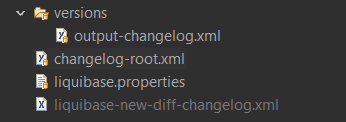
\includegraphics[width=9cm, height=3cm]{liquibase-changelog.png}
\caption{\label{datenbank:konfiguration} Liquibase-Konfiguration}
\end{figure}
\section*{\small \textbf{1. Liquibase Konfiguration - liquibase.properties}}
In dieser Datei werden allgemeine Einstellungen wie der Datenbankzugang und die zu verwendenden Changelog-Konfiguration festgelegt.
\begin{lstlisting}[language=properties]
# Database Configuration
url=jdbc:postgresql://192.168.252.140:5432/opendataconn_ng
username=opendataconn_ng_usr
password=
driver=org.postgresql.Driver
# Reference Configuration
referenceUrl=hibernate:spring:de.ahu.opendata?dialect=org.hibernate.dialect.PostgreSQLDialect
referenceDriver=liquibase.ext.hibernate.database.connection.HibernateDriver
# Output Files
changeLogFile=src/main/resources/db/changelog-root.xml
diffChangeLogFile=src/main/resources/db/liquibase-new-diff-changelog.xml
outputChangeLogFile=src/main/resources/db/versions/output-changelog.xml
\end{lstlisting}
\section*{\small \textbf{2. Changelog Konfiguration - changelog-root.xml}}
Ein so genannter Root-ChangeLog wird erstellt, welcher in XML geschrieben ist und eine output-changelog.xml inkludiert, welche im Ordner ,,versions'' zu finden ist. Diese Datei sorgt dafür, dass Liquibase das ChangeSet findet.
\begin{lstlisting}
<?xml version="1.0" encoding="UTF-8"?>   
<databaseChangeLog
   xmlns="http://www.liquibase.org/xml/ns/dbchangelog"
   xmlns:xsi="http://www.w3.org/2001/XMLSchema-instance"
   xmlns:pro="http://www.liquibase.org/xml/ns/pro"
   xsi:schemaLocation="http://www.liquibase.org/xml/ns/dbchangelog
      http://www.liquibase.org/xml/ns/dbchangelog/dbchangelog-4.23.xsd
      http://www.liquibase.org/xml/ns/pro 
      http://www.liquibase.org/xml/ns/pro/liquibase-pro-4.23.xsd">  
    <includeAll path="db/versions"/>  
</databaseChangeLog>
\end{lstlisting}
\section*{\small \textbf{3. Changelog Konfiguration - output-changelog.xml}}
Diese Datei enthält sämtliche Datenbankänderungen und die Änderungen werden in Form von ChangeSet beschrieben und verwaltet.Im Folgenden ist ein Abschnitt im XML-Format für das Anlagen einer Tabelle Abonnement wiedergegeben. \\ 
\begin{lstlisting}
<changeSet author="ng (generated)" id="1743435452264-1">
    <createTable tableName="abonnement">
        <column name="id" type="VARCHAR(32)">
            <constraints nullable="false" primaryKey="true" primaryKeyName="abonnementPK" />
        </column>
        <column name="description" type="TEXT" />
        <column name="label" type="VARCHAR(255)">
            <constraints nullable="false" />
        </column>
        <column name="base_url" type="VARCHAR(255)" />
        <column name="file_format" type="VARCHAR(255)" />
        <column name="end_datum" type="date" />
        <column name="location_id" type="VARCHAR(255)" />
        <column name="parameter" type="VARCHAR(255)" />
        <column name="start_datum" type="date" />
        <column name="sub_url" type="VARCHAR(255)" />
    </createTable>
</changeSet>
\end{lstlisting}
\section*{\small \textbf{4. Changelog Konfiguration - liquibase-new-diff-changelog.xml}}
Diese Datei enthält nur bestimmte Änderungen von bestimmten Tabellen, die man in die Datei \texttt{output-changelog.xml} einfügt, wenn man das Schema der Datenbank modifiziert. Ähnlich wie in \texttt{output-changelog.xml} werden Änderungen auch in Form von ChangeSet beschrieben.

\section{Datenbankmanagementsystem}
Wie bereits in dem letzten Abschnitt offengelegt, wird ein PostgreSQL als das Datenbankmanagementsystem gewählt. 
Da alle Datenbanken von Ahu GmbH zentral im lokalen Netzwerk liegen und die meisten Projekte PostgreSQL-Datenbank verwenden, ist es deswegen ersichtlich, dass für dieses Projekt auch eine PostgreSQL-Datenbank verwendet wird. \\
Außerdem spricht der Einsatz einer PostgreSQL-Datenbank aufgrund ihrer zahlreichen Vorteile für sich.
\begin{enumerate}
\item Open-Source: geringe Kosten und hohe Flexibilität und Innovation, die bei anderen Datenbanklösung nicht immer möglich sind. 
\item Leistung und Skalierbarkeit : PostgreSQL unterstützt eine Vielzahl von Leistungsoptimierung und verfügt über eine hohe Lese-/Schreibgeschwindigkeit, insbesondere bei der Unterstützung von Geodaten.
\item Fundierte Sprachunterstützung : Aufgrund seiner Kompatibilität und Unterstützung mehrerer Programmiersprachen ist PostgreSQL eine der flexibelsten Datenbanken für Entwickler. Python, JavaScript, C/C++, Java und weitere beliebte Programmiersprachen bieten ausgereifte Unterstützung für PostgreSQL.
\end{enumerate}

\chapter{Anforderungsanalyse und Spezifikation }
\section{Analyse}
Während der Analysephase werden die \textbf{\textit{Stakeholder}} identifiziert und deren Anforderungen mittels \textbf{\textit{User Stories}} gesammelt. Die Anforderungen können in drei verschiedenen Untergruppen eingeteilt werden, um die systematisch und spezifisch behandeln zu können.
\begin{enumerate}
\item Funktionale Anforderungen beschreiben die Funktionen, die eine ganze Anwendung oder auch nur eine von ihren Komponenten erfüllen soll. Eine Funktion besteht aus drei Schritten: Eingabe der Daten-Systemverhalten-Ausgabe der Daten. Sie kann die Daten berechnen und manipulieren, Geschäftsprozesse ausführen, Benutzerinteraktionen herstellen oder andere Aufgabe ausführen.
\item Nicht-funktionale Anforderungen beschreiben, wie das System es tut, während die funktionalen Anforderungen bestimmen, was das System tut. Darunter zählen die Leistungsstandards und Qualitätsmerkmale von Software, z.B. die Benutzerfreundlichkeit, Effektivität, Sicherheit, Skalierbarkeit usw.
\item Randbedingungen sind Vorgaben, die den Lösungsraum einschränken und das Verhalten der Software beeinflussen.
\end{enumerate}
\subsection{Anwendungsszenario}
Die zu entwickelnde Applikation soll als zentrale Stelle für die Durchsuche der Geodaten und Verwaltung der relevanten Geodaten dienen und ist auch in der Lage, diese Geodaten durch eine Schnittstelle einen anderen Client zur Verfügung stellen zu können.
\subsection{Stakeholder}
In der Softwareentwicklung sind Stakeholder Personen, Gruppen oder Organisation, die ein Interesse am Erfolg eines Softwareprojekts haben und von dessen Ergebnissen direkt oder indirekt beeinflusst werden.

\subsection{User-Stories}
Mittels User-Stories können funktionale Anforderungen der Stakeholder erfasst werden.
\begin{enumerate}
\item Als Benutzer möchte ich in der Web-Oberfläche eine Übersicht über populäre Datenquellen sehen, die  relevante Geodaten bereitstellen.
\item Als Benutzer möchte ich mithilfe von Schlagwörtern nach OGC-Webservices durchsuchen und die entsprechenden Referenzen als URL-Links zu den Schlagwörtern erhalten.
\item Als Benutzer möchte ich gezielt nach Messdaten wie Grundwasserständen, Pegelständen, Niederschlag, etc. recherchieren und dabei Informationen über das Datenformat und wesentliche Inhalte der Datensätze erhalten.
\item Als Benutzer möchte ich Messdaten, die meist im CSV-Format oder individuell strukturierte ASCII-Dateien vorliegen, in ein passendes Zielformat konvertieren lassen.
\item Als Benutzer möchte ich die Daten in Form einer List von Datenstreams angezeigt bekommen.
\item Als Benutzer möchte ich in der Lage sein, bestimmte Datensätze abonnieren zu können.
\item Als Benutzer möchte ich die gefundenen Geo- und Messdaten visuell auf einer Karte darstellen lassen.
\end{enumerate}

\section{Spezifikation}
Mit den im letzten Abschnitt erhobenen User-Stories können nun die funktionalen Anforderung genauer spezifiziert werden. Dort werden Use-Cases genauer definiert.
\subsection{Use-Cases}
Einfach ausgedrückt wird mit einem Use-Case die nach außen sichtbare Interaktion eines Nutzers mit einem System dokumentiert. Dieser Nutzer kann entweder eine Person, eine Organisation oder ein anderes System sein.\\
Für die prototypische Anwendung werden folgenden Use-Cases ausgearbeitet.
\section*{\small \textbf{Use-Case 1: Historische Wetterdaten von Wetterdatendienst einsehen}}
Akteur : Benutzer\\
Ziel: Historische Wetterdaten einer bestimmten Messtation einsehen\\
Vorbedingung: keine\\
Nachbedingung: keine\\
\underline{Ablauf}:
\begin{enumerate}
\item Benutzer navigiert zu der Historische Wetterdaten - Seite
\item Am Anfang zeigt die Seite einige Dropdowns zur Durchsuche der Daten und eine Karte, auf der noch keine Station zu sehen ist
\item Benutzer wählt die gewünschte Auflösung aus (stündlich, täglich, monatlich, jährlich)
\item Benutzer wählt dann die Hauptparameter aus und ein Dropdown für Unterparamter blendet sich ein.
\item Benutzer wählt anschließend die Unterparamter aus.
\item Das System reagiert auf den Wert von Unterparamter und zeigt sich eine deutschlandweite Karte, wo alle relevanten Messstationen zu dem ausgewählten Unterparamter zu sehen sind. 
\item Weitere Dropdowns werden danach eingeblendet, entweder möchte Benutzer die Messstationen in einem bestimmten Bundesland sehen oder direkt eine gezielte Messstation auswählen
\item Nach Auswahl einer Station wird die Station auf der Karte fokussiert und die Daten zur gewählten Station als Diagramm dargestellt. 
\end{enumerate}
\section*{\small \textbf{Use-Case 2: Wettervorhersagedaten von Wetterdatendienst einsehen}}
Akteur : Benutzer\\
Ziel:  Vorhersagedaten einer bestimmten Messtation einsehen\\
Vorbedingung: keine\\
Nachbedingung: keine\\
\underline{Ablauf}:
\begin{enumerate}
\item Benutzer navigiert zu der Wettervorhersage - Seite
\item Die Seite stellt bereits eine Tabelle mit verschiedenen Parameter zum Ansehen der Wetterdaten.
\item Benutzer wählt eine Station aus dem Dropdown aus.
\item Nach der Auswahl erscheint automatisch ein Button zur Überprüfung der Verfügbarkeit der Wetterdaten.
\item Benutzer klickt auf dieses Button und wartet auf die Meldung des Systems.
\item Das System überprüft all in der Grid befindliche Parameter,ob jeweiliger Parameter überhaupt Daten liefert. 
\item Anhand des Status,ob es die Daten zu jeweiligen Parameter gibt, wird es in der Grid ein weitere Spalte zur Einsicht der Daten geben. 
\item Benutzer klickt auf das Icon in der neu erscheinenden Spalte.
\item Ein Fenster öffnet sich und stellt die Daten in Form eines Diagramm bereits. 
\end{enumerate}
\section*{\small \textbf{Use-Case 3: Pegelstanddaten von \href{https://www.pegelonline.wsv.de/gast/start} {PegelOnline} einsehen}}
\begin{enumerate}
\item Benutzer navigiert zu der Pegelständedaten - Seite
\item Benutzer sieht eine Karte mit Pegelstationen deutschlandweit, die je nach aktueller Lage farblich kategorisiert sind.
\item 
	Inhalt...
\end{enumerate}


\section*{\small \textbf{Use-Case 4:}}


\chapter{Konzeption und Architektur}

\chapter{Implementierung}

\chapter{Evaluierung}

\chapter{Fazit und Ausblick}

\printbibliography
\end{document}